\documentclass{article}

% NeurIPS 2026 — preprint mode (no anonymous, shows authors)
\usepackage[preprint]{neurips_2026}

% ── Encoding & fonts ─────────────────────────────────────────────────────────
\usepackage[utf8]{inputenc}
\usepackage[T1]{fontenc}

% ── Core packages ─────────────────────────────────────────────────────────────
\usepackage{hyperref}
\usepackage{url}
\usepackage{booktabs}
\usepackage{amsmath}
\usepackage{amsfonts}
\usepackage{amssymb}
\usepackage{nicefrac}
\usepackage{microtype}
\usepackage{xcolor}
\usepackage{graphicx}
\usepackage{multirow}
\usepackage{array}
\usepackage{enumitem}
\usepackage{caption}
\usepackage{subcaption}

% ── TikZ for figures ──────────────────────────────────────────────────────────
\usepackage{tikz}
\usetikzlibrary{arrows.meta, positioning, shapes.geometric,
                fit, backgrounds, calc}

% ── Hyperref colours ──────────────────────────────────────────────────────────
\hypersetup{
  colorlinks = true,
  linkcolor  = blue!70!black,
  citecolor  = blue!55!black,
  urlcolor   = blue!55!black
}

% ── Convenience macros ────────────────────────────────────────────────────────
\newcommand{\nerf}{NeRF}
\newcommand{\tgs}{3DGS}
\newcommand{\nvs}{NVS}
\newcommand{\wm}{World Model}
\newcommand{\todo}[1]{\textcolor{red}{[TODO: #1]}}
\newcommand{\etal}{\emph{et al.}}
\newcommand{\ie}{\emph{i.e.}}
\newcommand{\eg}{\emph{e.g.}}

% ─────────────────────────────────────────────────────────────────────────────
%  TITLE / AUTHORS
% ─────────────────────────────────────────────────────────────────────────────
\title{%
  Towards Generative World Modeling: \\
  A Comprehensive Survey for Novel View Synthesis%
}

\author{%
  ElephantFlow Research \\
  \texttt{\href{https://github.com/elephantflow/ElephantSurvey}{%
    github.com/elephantflow/ElephantSurvey}} \\[2pt]
  \textit{Draft v0.1 — March 2026}
}

% ═════════════════════════════════════════════════════════════════════════════
\begin{document}
\maketitle

% ─────────────────────────────────────────────────────────────────────────────
%  ABSTRACT
% ─────────────────────────────────────────────────────────────────────────────
\begin{abstract}
Novel View Synthesis~(\nvs{})---the task of rendering a scene from arbitrary
unseen viewpoints given a set of reference observations---has undergone a
paradigm shift from classical geometry-based reconstruction toward
learning-driven generative approaches.
This survey examines \nvs{} not merely as a rendering technique, but as the
\textbf{foundational spatial capability} of Generative World Models:
systems that predict visual scene states under arbitrary conditions, including
viewpoint changes, temporal dynamics, and agent interactions.
We provide a comprehensive review spanning three dominant paradigms---%
\emph{implicit neural representations}~(\nerf{} and variants),
\emph{explicit Gaussian-based representations}~(\tgs{} and variants),
and \emph{generative model-driven synthesis} (diffusion models and score
distillation methods)---and analyse how each advances, or falls short of, the
full demands of world modelling.
We further survey emerging 4D approaches that unify spatial and temporal
prediction, and identify key open challenges including physical consistency,
scalable generalisation, and the geometry--generation trade-off.
Our analysis reveals that the field is at a critical inflection point where
\nvs{} and world modelling are converging, and we lay out a research roadmap
toward truly generalisable, physically grounded world models.
\end{abstract}

% ─────────────────────────────────────────────────────────────────────────────
%  1. INTRODUCTION
% ─────────────────────────────────────────────────────────────────────────────
\section{Introduction}
\label{sec:intro}

\subsection{The Fundamental Challenge}

Intelligence, whether biological or artificial, requires the ability to reason
about the world beyond what is immediately visible.
A surgeon planning an incision must mentally rotate a 3-D anatomy from a 2-D
scan.
A self-driving vehicle must anticipate occlusion from a new perspective before
rounding a corner.
A robot must predict how a grasped object will appear from the wrist camera
before it reaches the target pose.
In each case the core cognitive operation is the same:
\textbf{synthesising a plausible visual state of the world at an unobserved
vantage point}.

This is the problem of \textbf{Novel View Synthesis~(\nvs{})}.
Formally, given a set of reference images
$\{\mathbf{I}_1,\ldots,\mathbf{I}_n\}$ captured from known camera poses
$\{\boldsymbol{\pi}_1,\ldots,\boldsymbol{\pi}_n\}$, the goal is to render a
photo-realistic image $\hat{\mathbf{I}}$ at an arbitrary target pose
$\boldsymbol{\pi}^{*}$, faithfully preserving scene geometry, appearance, and
lighting.

While the problem was articulated decades ago in the image-based rendering
literature~\citep{levoy1996light,mcmillan1995plenoptic}, the past five years
have witnessed an extraordinary leap in capability driven by deep learning,
differentiable rendering, and generative modelling.
Yet despite remarkable progress, a critical question remains underexplored:
\emph{in what sense does a system that can synthesise novel views ``understand''
the world?}
And conversely, \emph{what must \nvs{} methods ultimately become in order to
serve as the spatial backbone of a true \wm{}?}

This survey is organised around these questions.
We treat \nvs{} not as an isolated rendering task, but as the
\textbf{spatial prediction axis} of a larger problem:
\textbf{Generative World Modelling}.

\subsection{What Is a World Model?}

\begin{quote}
  \textbf{Working Definition.}\quad
  A \emph{\wm{}} is a learned system that can predict the visual (and
  optionally physical) state of a scene under arbitrary conditions---including
  viewpoint changes, temporal evolution, and agent-driven interactions---in a
  manner that is \emph{geometrically consistent}, \emph{physically plausible},
  and \emph{generalisable} beyond the training distribution.
\end{quote}

This definition deliberately extends the classic control-theoretic
formulation~\citep{ha2018worldmodels,lecun2022path}, where a world model
predicts the next latent state given an action.
We expand the ``condition'' axis to include camera pose as a first-class
citizen, making \nvs{} a natural special case: when the condition is a
viewpoint change and the scene is static, the world model reduces exactly to
an \nvs{} system.

Conversely, a world model must go beyond \nvs{} in two critical dimensions.
(1)~\textbf{Temporal prediction}: a world model must handle dynamic scenes,
predicting how the scene evolves over time under physics, agent actions, or
autonomous dynamics---static \nvs{} methods cannot address this axis.
(2)~\textbf{Action conditioning}: a world model must be \emph{controllable};
given an agent action (move forward, grasp, rotate), it must render the
resulting observation, requiring semantic and physical understanding beyond
geometric interpolation.

\subsection{Why \nvs{} Is the Core of World Modelling}

Among all world model capabilities, \textbf{spatial consistency} is the
foundational constraint.
A temporal prediction that is geometrically inconsistent---where a coffee mug
occupies two different positions when viewed from two angles---is not a world
model; it is a hallucination.
\nvs{} is precisely the discipline that enforces multi-view geometric
consistency, making it a non-negotiable prerequisite for any credible world
model.

\medskip
\noindent\textbf{Central Thesis.}\quad
\textit{\nvs{} is the spatial inference engine of world modelling.
Without it, a ``world model'' reduces to a video generator---capable of
producing plausible-looking sequences but unable to support downstream tasks
that require spatial grounding, such as robot manipulation, surgical planning,
or autonomous navigation.}
\medskip

Advances in \nvs{}---from dense input to sparse-view generalisation, from
static scenes to dynamic 4-D modelling---map directly onto advances in world
modelling capability.
We use this lens throughout the survey to evaluate each method: not only by
its PSNR on standard benchmarks, but by its contribution toward five
world-modelling desiderata (Section~\ref{sec:background}).

\subsection{The Evolution Arc: From Reconstruction to Generation}

The history of \nvs{} can be understood as a progressive relaxation of input
constraints, each step demanding stronger scene priors and thus moving closer
to generative world modelling (see Table~\ref{tab:evolution}).

\begin{table}[t]
  \centering
  \caption{%
    Four eras of Novel View Synthesis characterised by dominant scene
    representation, input regime, and chief world-modelling limitation.%
  }
  \label{tab:evolution}
  \small
  \setlength{\tabcolsep}{4pt}
  \begin{tabular}{@{}lllll@{}}
    \toprule
    \textbf{Era} & \textbf{Period} & \textbf{Representation}
      & \textbf{Input} & \textbf{Chief Limitation} \\
    \midrule
    I   & 2015--2020 & Explicit mesh / light field
        & Dense multi-view   & No learning prior; brittle \\
    II  & 2020--2023 & Implicit MLP~(\nerf{})
        & Dense $\to$ sparse & Per-scene; slow \\
    III & 2023--now  & Explicit Gaussians~(\tgs{})
        & Dense; feed-fwd    & Reconstruction-centric \\
    IV  & 2022--now  & Diffusion / score distillation
        & Single image/text  & Geometry--generation gap \\
    \bottomrule
  \end{tabular}
\end{table}

\paragraph{Era~I (2015--2020): Classical Reconstruction.}
Structure-from-Motion~(SfM), multi-view stereo~(MVS), and light-field methods
dominated~\citep{schoenberger2016sfm}.
High-quality outputs were achievable under tightly controlled conditions, but
no generative prior was available and dense input was mandatory.

\paragraph{Era~II (2020--2023): Neural Radiance Fields.}
Mildenhall~\etal~\citep{mildenhall2020nerf} introduced \nerf{}: a continuous
implicit scene representation encoded in an MLP, trained via differentiable
volume rendering.
The community rapidly extended \nerf{} to dynamic deformations~%
\citep{park2021nerfies,pumarola2021dnerf}, unbounded scenes, and
cross-scene generalisation~\citep{yu2021pixelnerf,wang2021ibrnet}.
Quality surpassed classical methods by large margins; the key limitation was
per-scene optimisation taking hours to days.

\paragraph{Era~III (2023--present): 3D Gaussian Splatting.}
Kerbl~\etal~\citep{kerbl2023gaussian} replaced the implicit MLP with
anisotropic Gaussian primitives rendered via differentiable rasterisation,
enabling real-time, high-fidelity rendering.
The community extended \tgs{} to dynamic scenes~%
\citep{wu2024_4dgs,yang2024spacetime} and feed-forward
generalisation~\citep{charatan2024pixelsplat,chen2024mvsplat}.
The paradigm remains reconstruction-centric with a weak generative prior.

\paragraph{Era~IV (2022--present): Generative Model-Driven \nvs{}.}
Diffusion models and score distillation methods~%
\citep{poole2023dreamfusion,liu2023zero1to3,gao2024cat3d,wu2024reconfusion}
enable \nvs{} from single images or text prompts.
Video diffusion models~%
\citep{agarwal2025cosmos,parkerholder2024genie2,yu2024viewcrafter}
unify temporal and viewpoint prediction, arriving at nascent 4-D World Models.

\medskip
Each era coexists with the others, addressing different points on the
trade-off frontier among reconstruction fidelity, input efficiency,
generalisation, and computational cost.
The current frontier lies in \textbf{integrating the geometric precision of
\nerf{}/\tgs{} with the generative priors of diffusion models}, while
extending both along the temporal axis---the path towards Generative World
Modelling.

\subsection{Existing Gaps}
\label{sec:intro:gaps}

Table~\ref{tab:gaps} summarises the capability landscape.
No single existing paradigm satisfies all world-model requirements:
reconstruction-based methods excel at geometric consistency but lack
generative priors; generative methods provide strong priors but sacrifice
geometric rigour.

\begin{table}[t]
  \centering
  \caption{%
    Capability coverage across \nvs{} paradigms against world-model
    requirements.
    \textbf{+}~achieved;\; $\sim$~partially/method-dependent;\;
    \textbf{--}~not addressed.%
  }
  \label{tab:gaps}
  \small
  \setlength{\tabcolsep}{4.5pt}
  \begin{tabular}{@{}lc@{\quad}c@{\quad}c@{\quad}c@{\quad}c@{}}
    \toprule
    \textbf{Capability}
      & \textbf{Classical}
      & \textbf{\nerf{}}
      & \textbf{\tgs{}}
      & \textbf{Gen.\ \nvs{}}
      & \textbf{Target} \\
    \midrule
    Geometric consistency       & + & + & + & $\sim$ & + \\
    Sparse/single-image input   & -- & $\sim$ & $\sim$ & + & + \\
    Dynamic scene (4-D)         & -- & $\sim$ & $\sim$ & $\sim$ & + \\
    Action/agent control        & -- & -- & -- & $\sim$ & + \\
    Physical plausibility       & -- & -- & -- & $\sim$ & + \\
    Cross-scene generalisation  & -- & $\sim$ & $\sim$ & + & + \\
    Real-time rendering         & $\sim$ & -- & + & -- & + \\
    \bottomrule
  \end{tabular}
\end{table}

\subsection{Contributions}
\label{sec:intro:contrib}

\begin{enumerate}[leftmargin=*, label=(\arabic*)]

  \item \textbf{A World-Modelling Lens for \nvs{}.}
    We introduce a unified analytical framework evaluating \nvs{} methods on
    five world-modelling desiderata: geometric consistency, generalisation,
    dynamic modelling, physical plausibility, and action controllability.

  \item \textbf{Comprehensive Taxonomy Across Three Paradigms.}
    We survey more than 150 methods spanning classical reconstruction, \nerf{}
    variants, \tgs{} variants, and generative \nvs{} approaches, analysing
    each method's representation, input regime, rendering mechanism, and
    world-modelling implications.

  \item \textbf{The 4-D Convergence Thesis.}
    We articulate and substantiate the claim that the field is converging
    toward 4-D World Modelling---the unification of spatial (\nvs{}) and
    temporal (video prediction) generation---and trace the technical
    developments driving this convergence.

  \item \textbf{Open Problems and Research Roadmap.}
    We identify the geometry--generation trade-off, long-horizon temporal
    consistency, physical grounding, and evaluation methodology as critical
    open problems, and propose a concrete research roadmap.

\end{enumerate}

\subsection{Paper Structure}

Section~\ref{sec:background} provides background: camera models,
differentiable volume rendering, and the unified \nvs{} formulation.
Section~\ref{sec:nerf} reviews implicit neural representations (\nerf{}).
Section~\ref{sec:3dgs} covers explicit Gaussian representations (\tgs{}).
Section~\ref{sec:generative} surveys generative \nvs{} approaches.
Section~\ref{sec:world} synthesises these into the world-modelling perspective.
Section~\ref{sec:datasets} reviews datasets and benchmarks.
Section~\ref{sec:open} identifies open problems and presents the roadmap.
Section~\ref{sec:conclusion} concludes.

% ─────────────────────────────────────────────────────────────────────────────
%  2. BACKGROUND
% ─────────────────────────────────────────────────────────────────────────────
\section{Background and Problem Formulation}
\label{sec:background}

\subsection{Camera Model}

We adopt the standard pinhole camera model.
A 3-D point $\mathbf{X} \in \mathbb{R}^3$ is projected to a 2-D pixel
$\mathbf{p} \in \mathbb{R}^2$ via
\begin{equation}
  \mathbf{p} = \mathbf{K}\,[\,\mathbf{R}\;\mathbf{t}\,]\,\tilde{\mathbf{X}},
  \label{eq:camera}
\end{equation}
where $\mathbf{K}$ is the $3{\times}3$ intrinsic matrix,
$\mathbf{R} \in \mathrm{SO}(3)$ and $\mathbf{t} \in \mathbb{R}^3$ define
the extrinsic pose, and $\tilde{\mathbf{X}}$ denotes homogeneous coordinates.
A camera ray emitted from the optical centre $\mathbf{o}$ along direction
$\mathbf{d}$ is parameterised as
$\mathbf{r}(s) = \mathbf{o} + s\,\mathbf{d}$, $s \in [s_n, s_f]$.

\subsection{Volume Rendering}

\nerf{}~\citep{mildenhall2020nerf} represents a scene as a continuous
radiance field $F_\theta: (\mathbf{x}, \mathbf{d}) \mapsto (\mathbf{c},
\sigma)$, where $\mathbf{c} \in \mathbb{R}^3$ is emitted colour and
$\sigma \geq 0$ is volume density.
The expected colour of a ray $\mathbf{r}$ is computed via the
\emph{volume rendering integral}:
\begin{equation}
  \hat{C}(\mathbf{r}) =
  \int_{s_n}^{s_f}
    T(s)\,\sigma\!\left(\mathbf{r}(s)\right)\,
    \mathbf{c}\!\left(\mathbf{r}(s),\mathbf{d}\right)
  \,\mathrm{d}s,
  \label{eq:volrender}
\end{equation}
where the transmittance
$T(s) = \exp\!\left(-\int_{s_n}^{s}\sigma(\mathbf{r}(u))\,\mathrm{d}u\right)$
accounts for accumulated occlusion.
In practice Eq.~\eqref{eq:volrender} is approximated by stratified sampling
and quadrature.

\subsection{Differentiable Rasterisation (\tgs{})}

\tgs{}~\citep{kerbl2023gaussian} represents a scene as a set of
$N$ anisotropic 3-D Gaussians
$\{\mu_i, \Sigma_i, \alpha_i, \mathbf{c}_i\}_{i=1}^{N}$,
where $\mu_i \in \mathbb{R}^3$ is the mean, $\Sigma_i$ the covariance,
$\alpha_i \in [0,1]$ the opacity, and $\mathbf{c}_i$ the (view-dependent)
colour encoded as spherical harmonics.
For a given viewpoint, each Gaussian is projected to a 2-D splat and
composited front-to-back:
\begin{equation}
  \hat{C} = \sum_{i \in \mathcal{N}}
    \mathbf{c}_i\,\alpha_i\,\tilde{G}_i
    \prod_{j < i} \left(1 - \alpha_j\,\tilde{G}_j\right),
  \label{eq:splatting}
\end{equation}
where $\tilde{G}_i$ is the 2-D Gaussian evaluated at the pixel centre.
Because all operations are differentiable, $\Sigma_i$, $\alpha_i$, and
$\mathbf{c}_i$ are optimised by gradient descent on photometric loss.

\subsection{Unified \nvs{} Formulation}

We define \nvs{} as the problem of learning a mapping
\begin{equation}
  \mathcal{M}_\theta:\;
  \bigl(\{\mathbf{I}_i, \boldsymbol{\pi}_i\}_{i=1}^{n},\;
         \boldsymbol{\pi}^{*}\bigr)
  \;\longrightarrow\;
  \hat{\mathbf{I}}^{*},
  \label{eq:nvs}
\end{equation}
where $n$ ranges from dense multi-view ($n \gg 1$) down to a single image
($n=1$), and $\boldsymbol{\pi}^{*}$ is the target camera pose.
The world-modelling extension augments Eq.~\eqref{eq:nvs} with a time index
$t$ and an action sequence $\mathbf{a}_{0:t}$:
\begin{equation}
  \mathcal{M}_\theta:\;
  \bigl(\{\mathbf{I}_i, \boldsymbol{\pi}_i\}_{i=1}^{n},\;
         \mathbf{a}_{0:t},\; t,\; \boldsymbol{\pi}^{*}\bigr)
  \;\longrightarrow\;
  \hat{\mathbf{I}}^{*}_t.
  \label{eq:wm}
\end{equation}
This unified formulation makes explicit the five world-modelling desiderata:
\textbf{(D1)}~geometric consistency across $\boldsymbol{\pi}^{*}$;
\textbf{(D2)}~generalisation to unseen scenes ($n \leq 1$);
\textbf{(D3)}~dynamic scene modelling ($t > 0$);
\textbf{(D4)}~action conditioning ($\mathbf{a}_{0:t} \neq \varnothing$);
\textbf{(D5)}~physical plausibility.

% ─────────────────────────────────────────────────────────────────────────────
%  3. NeRF
% ─────────────────────────────────────────────────────────────────────────────
\section{Implicit Neural Representations: \nerf{} and Variants}
\label{sec:nerf}

\subsection{Original \nerf{}}

Mildenhall~\etal~\citep{mildenhall2020nerf} encode a static scene in the
weights of an MLP $F_\theta$ that maps a 5-D input---3-D position
$\mathbf{x}$ and 2-D viewing direction $\mathbf{d}$---to colour $\mathbf{c}$
and density $\sigma$.
Positional encoding $\gamma(\mathbf{x})$ lifts inputs to a higher-frequency
space, enabling the MLP to represent fine geometric detail.
Training minimises a photometric reconstruction loss over held-out pixels via
the volume rendering integral~(Eq.~\ref{eq:volrender}).

\paragraph{World-Modelling Implications.}
\nerf{} achieves strong geometric consistency~(D1) but satisfies none of the
other desiderata: per-scene optimisation precludes generalisation~(D2),
the static assumption rules out dynamics~(D3) and action conditioning~(D4),
and no physical prior is enforced~(D5).

\subsection{Acceleration Methods}
\label{sec:nerf:accel}

Vanilla \nerf{} requires thousands of network evaluations per ray and hours
of training.
Three complementary strategies have been pursued.

\paragraph{Explicit grid hybrids.}
Plenoxels~\citep{fridovich2022plenoxels} and
TensoRF~\citep{chen2022tensorf} replace the MLP with sparse voxel grids or
tensor decompositions, reducing training to minutes while maintaining quality.

\paragraph{Hash-based encodings.}
Instant-NGP~\citep{muller2022instant} uses a multi-resolution hash grid to
achieve sub-second training, enabling interactive scene capture.

\paragraph{Knowledge distillation / baking.}
Methods such as MobileNeRF~\citep{chen2023mobilenerf} distil a trained \nerf{}
into a mesh-texture representation, enabling real-time rendering on commodity
hardware.

\subsection{Generalisation Methods}
\label{sec:nerf:general}

The per-scene limitation of vanilla \nerf{} has been addressed by
conditioning the network on image features extracted from reference views.

\textbf{pixelNeRF}~\citep{yu2021pixelnerf} conditions $F_\theta$ on pixel-aligned
image features from a CNN encoder, enabling single-image~(D2) reconstruction.
\textbf{IBRNet}~\citep{wang2021ibrnet} aggregates features from multiple reference
views via cross-attention, generalising to novel scenes at test time.
\textbf{MVSNeRF}~\citep{chen2021mvsnerf} constructs a cost volume from multi-view
stereo and conditions the radiance field on this volume, combining geometric
priors with learned appearance.

\subsection{Dynamic \nerf{}}
\label{sec:nerf:dynamic}

Extending \nerf{} to dynamic scenes addresses desideratum~D3.

\textbf{D-NeRF}~\citep{pumarola2021dnerf} introduces a deformation network that
maps each time-stamped point to a canonical space, where a standard \nerf{} is
evaluated.
\textbf{Nerfies}~\citep{park2021nerfies} and
\textbf{HyperNeRF}~\citep{park2021hypernerf} model more complex non-rigid
deformations via latent deformation codes and higher-dimensional ambient
spaces, respectively.
\textbf{K-Planes}~\citep{fridovich2023kplanes} decomposes the 4-D space-time
radiance field into six orthogonal feature planes, enabling efficient
optimisation of dynamic scenes.

\paragraph{World-Modelling Implications.}
Dynamic \nerf{} methods achieve~D3, but per-scene optimisation still
precludes generalisation~(D2), and action conditioning~(D4) remains absent.

% ─────────────────────────────────────────────────────────────────────────────
%  4. 3DGS
% ─────────────────────────────────────────────────────────────────────────────
\section{Explicit Gaussian Representations: \tgs{} and Variants}
\label{sec:3dgs}

\subsection{3D Gaussian Splatting}

Kerbl~\etal~\citep{kerbl2023gaussian} initialise Gaussians from an SfM point
cloud and optimise them jointly via the differentiable splatting render
(Eq.~\ref{eq:splatting}).
An adaptive densification strategy adds Gaussians in under-reconstructed
regions and prunes low-opacity ones, yielding compact representations.
Real-time rendering at ${\sim}100$~fps at 1080p is achieved on a modern GPU.

\paragraph{World-Modelling Implications.}
\tgs{} achieves strong geometric consistency~(D1) and real-time rendering, a
prerequisite for interactive world models.
However, like \nerf{}, it is per-scene optimised and lacks generative priors,
leaving D2--D5 unaddressed.

\subsection{Dynamic Extensions}
\label{sec:3dgs:dynamic}

\textbf{4D Gaussian Splatting~(4DGS)}~\citep{wu2024_4dgs} extends Gaussians
into a 4-D space-time representation, coupling each Gaussian with a time-varying
deformation field.
\textbf{SpacetimeGaussians}~\citep{yang2024spacetime} parameterise Gaussian
trajectories as polynomial functions of time, enabling smooth interpolation
across frames.
Both methods deliver real-time dynamic rendering, advancing~D3 while
retaining~D1.

\subsection{Feed-Forward Generalisation}
\label{sec:3dgs:generalise}

Combining the efficiency of Gaussian splatting with the generalisation of
learned priors has been a major recent thrust.

\textbf{pixelSplat}~\citep{charatan2024pixelsplat} predicts per-pixel Gaussian
parameters from an image-pair encoder, enabling single-forward-pass \tgs{}
reconstruction for novel scene pairs~(D2).
\textbf{MVSplat}~\citep{chen2024mvsplat} extends this to sparse multi-view inputs
using a cost-volume prior, improving geometric accuracy.
\textbf{Splatt3R}~\citep{smart2024splatt3r} builds on the DUSt3R framework to
predict scene-consistent Gaussians from unposed image pairs.

\paragraph{World-Modelling Implications.}
Feed-forward \tgs{} methods simultaneously address~D1 and~D2, a significant
step.
Dynamics (D3) and action conditioning~(D4) remain active research targets.

% ─────────────────────────────────────────────────────────────────────────────
%  5. GENERATIVE APPROACHES
% ─────────────────────────────────────────────────────────────────────────────
\section{Generative Approaches to \nvs{}}
\label{sec:generative}

\subsection{3-D-Aware Generative Adversarial Networks}
\label{sec:generative:gan}

Before diffusion models, GAN-based methods pioneered the integration of
generative priors with 3-D scene representations.
\textbf{GRAF}~\citep{schwarz2020graf} and
\textbf{pi-GAN}~\citep{chan2021pigan} condition a radiance-field generator on
a latent code, enabling multi-view consistent image synthesis from a single
code without real 3-D supervision.
\textbf{EG3D}~\citep{chan2022efficient} introduces the tri-plane representation,
encoding a scene on three orthogonal feature planes and decoding with a shallow
MLP, dramatically improving quality and training speed.

\paragraph{World-Modelling Implications.}
These methods demonstrate that strong generative priors can enforce
multi-view consistency (D1) while supporting cross-identity generalisation
(D2 for objects), but they do not address dynamics (D3) or action
conditioning (D4).

\subsection{Diffusion-Based \nvs{}}
\label{sec:generative:diffusion}

Diffusion models have rapidly become the dominant generative backbone for
\nvs{}, owing to their superior sample quality and ability to incorporate
conditioning signals.

\textbf{Zero-1-to-3}~\citep{liu2023zero1to3} fine-tunes a latent diffusion
model~\citep{rombach2022ldm} on multi-view object datasets, conditioning
the denoising process on a relative camera pose.
At inference, a single RGB image suffices to synthesise novel views~(D2),
though geometric consistency across multiple synthesised views is limited.

\textbf{One-2-3-45}~\citep{liu2023one2345} addresses this by lifting diffusion
multi-view outputs into a consistent 3-D reconstruction, combining the
generative prior of Zero-1-to-3 with reconstruction-based consistency.

\textbf{SyncDreamer}~\citep{liu2023syncdreamer} enforces 3-D consistency
explicitly by jointly denoising multiple views with shared 3-D attention,
producing geometrically coherent multi-view outputs from a single image.

\textbf{Cat3D}~\citep{gao2024cat3d} and
\textbf{ReconFusion}~\citep{wu2024reconfusion} extend the idea to sparse-view
inputs: a multi-view diffusion model generates additional views, which are
then fused via \nerf{} or \tgs{} into a complete 3-D scene.

\paragraph{World-Modelling Implications.}
Diffusion-based methods make substantial progress on D2 (sparse/single-image
input) but trade geometric rigour for generative flexibility, leaving a
geometry--generation gap.

\subsection{Score Distillation Sampling}
\label{sec:generative:sds}

Score Distillation Sampling~(SDS), introduced in
\textbf{DreamFusion}~\citep{poole2023dreamfusion}, optimises a 3-D
representation (originally \nerf{}, later \tgs{}) so that renders from all
viewpoints score highly under a pre-trained 2-D diffusion model.
This sidesteps the need for multi-view training data and opens the door to
text-driven 3-D generation.

\textbf{Magic3D}~\citep{lin2023magic3d} and
\textbf{ProlificDreamer}~\citep{wang2023prolificdreamer} address the over-smoothing
artefacts of vanilla SDS via coarse-to-fine strategies and variational
score distillation, respectively.
\textbf{GaussianDreamer}~\citep{yi2024gaussiandreamer} combines SDS with \tgs{}
initialisation for faster, higher-quality text-to-3D.

\paragraph{World-Modelling Implications.}
SDS-based methods achieve open-vocabulary 3-D generation (a form of D2) and
begin to encode semantic knowledge, but geometric fidelity remains below
reconstruction-based methods.

\subsection{Video Diffusion for 4-D \nvs{}}
\label{sec:generative:video}

The most direct path to generative world modelling is to unify spatial and
temporal generation in a single model.

\textbf{ViewCrafter}~\citep{yu2024viewcrafter} conditions a video diffusion
model on camera trajectories, generating temporally coherent novel-view
sequences from sparse input images.
\textbf{Cosmos}~\citep{agarwal2025cosmos} is a large-scale video generation
foundation model trained on internet-scale video, demonstrating emergent 3-D
consistency and physical plausibility.
\textbf{Genie~2}~\citep{parkerholder2024genie2} is an interactive world model
that generates playable 3-D environments conditioned on actions, directly
targeting~D4.

\paragraph{World-Modelling Implications.}
These methods are the closest current approximations to the generalised world
model of Eq.~\eqref{eq:wm}, partially satisfying D1--D4.
Physical plausibility~(D5) and long-horizon coherence remain the primary
open challenges.

% ─────────────────────────────────────────────────────────────────────────────
%  6. TOWARDS WORLD MODELLING
% ─────────────────────────────────────────────────────────────────────────────
\section{Towards World Modelling: 4-D and Beyond}
\label{sec:world}

\subsection{The 4-D Convergence Thesis}

We observe a clear convergence: the \nvs{} community is progressively
incorporating the temporal axis, while the world-modelling community is
increasingly adopting explicit 3-D representations for spatial grounding.
The meeting point is \textbf{4-D World Modelling}: a system that generates
geometrically consistent, temporally coherent, and physically plausible
scene observations under arbitrary viewpoint and action conditions.

Figure~\ref{fig:convergence} illustrates this convergence schematically.

\begin{figure}[t]
  \centering
  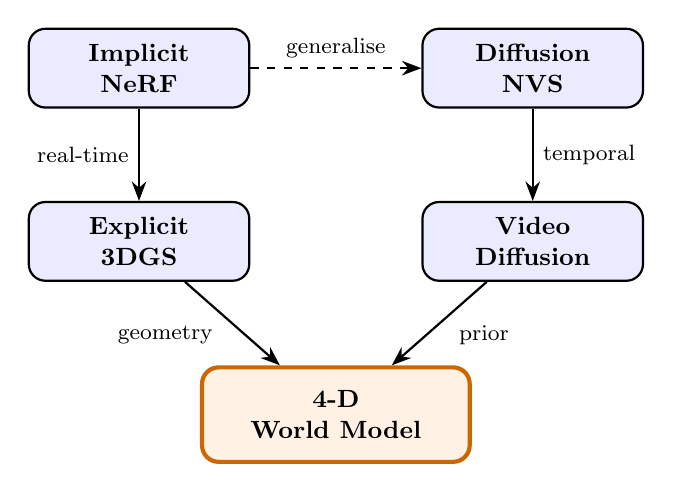
\begin{tikzpicture}[
      era/.style  = {rounded corners=6pt, draw, thick, fill=blue!8,
                     minimum width=2.8cm, minimum height=1cm,
                     font=\small\bfseries, align=center},
      arrow/.style= {-{Stealth[length=7pt]}, thick},
      target/.style= {rounded corners=6pt, draw=orange!80!black,
                      line width=1.5pt, fill=orange!10,
                      minimum width=3.4cm, minimum height=1.2cm,
                      font=\small\bfseries, align=center}
    ]
    \node[era]  (nerf)  at (0,2.2)   {Implicit\\\nerf{}};
    \node[era]  (3dgs)  at (0,0)     {Explicit\\\tgs{}};
    \node[era]  (diff)  at (5,2.2)   {Diffusion\\NVS};
    \node[era]  (video) at (5,0)     {Video\\Diffusion};
    \node[target](wm)   at (2.5,-2.2){4-D\\World Model};

    \draw[arrow] (nerf)  -- node[left,  font=\footnotesize]{real-time} (3dgs);
    \draw[arrow] (diff)  -- node[right, font=\footnotesize]{temporal}  (video);
    \draw[arrow] (3dgs)  -- node[below left,  font=\footnotesize, pos=0.4]{geometry} (wm);
    \draw[arrow] (video) -- node[below right, font=\footnotesize, pos=0.4]{prior} (wm);
    \draw[arrow, dashed] (nerf)  -- node[above, font=\footnotesize]{generalise} (diff);
  \end{tikzpicture}
  \caption{%
    The 4-D Convergence: reconstruction-based \nvs{} (left column) provides
    geometric rigour; generative \nvs{} (right column) provides visual priors.
    Both streams are converging toward 4-D World Modelling (bottom).%
  }
  \label{fig:convergence}
\end{figure}

\subsection{Embodied and Driving Applications}

The practical urgency of world modelling is clearest in embodied AI and
autonomous driving.

\textbf{UniSim}~\citep{yang2023unisim} models urban driving scenes as neural
closed-loop sensor simulators, rendering novel viewpoints for policy training
and evaluation.
\textbf{GAIA-1}~\citep{hu2023gaia} learns a generative world model of driving
conditioned on ego-actions, video, and text, enabling diverse scenario
generation for autonomous vehicle training.
Both works underscore that \nvs{} capabilities are the bottleneck: without
geometrically faithful viewpoint synthesis, simulated training data fails to
transfer to real deployment.

\subsection{Interactive World Generation}

Genie~2~\citep{parkerholder2024genie2} generates persistent, interactive 3-D
environments from a single image prompt, supporting first-person navigation and
object interaction.
Cosmos~\citep{agarwal2025cosmos} scales this to physical world simulation,
demonstrating that internet-scale video pre-training can instil emergent 3-D
consistency and physics priors.
These results suggest that the boundary between \nvs{} and world modelling is
already dissolving at the frontier.

% ─────────────────────────────────────────────────────────────────────────────
%  7. DATASETS AND BENCHMARKS
% ─────────────────────────────────────────────────────────────────────────────
\section{Datasets and Benchmarks}
\label{sec:datasets}

\subsection{Static Scene Benchmarks}

\textbf{NeRF-Synthetic}~\citep{mildenhall2020nerf}: eight synthetic objects
with known ground-truth, widely used for controlled \nvs{} evaluation.
\textbf{LLFF}~\citep{mildenhall2019llff}: forward-facing real scenes; tests
interpolation quality.
\textbf{Tanks and Temples}~\citep{knapitsch2017tanks}: large-scale unbounded
outdoor and indoor scenes with LiDAR ground truth.
\textbf{DTU}~\citep{jensen2014dtu}: multi-view stereo benchmark with object-level
scenes and calibrated illumination.
\textbf{Mip-NeRF~360}~\citep{barron2022mipnerf360}: unbounded 360$^\circ$ real
scenes with complex backgrounds.

\subsection{Dynamic Scene Benchmarks}

\textbf{D-NeRF dataset}~\citep{pumarola2021dnerf}: six monocular synthetic
dynamic scenes.
\textbf{NHR}~\citep{wu2020nhr}: multi-view video of human performance.
\textbf{CMU Panoptic Studio}~\citep{joo2015panoptic}: dense multi-view captures
of human activities with body pose annotations.

\subsection{Large-Scale and Outdoor}

\textbf{Waymo Open Dataset}~\citep{sun2020waymo} and
\textbf{nuScenes}~\citep{caesar2020nuscenes}: autonomous driving datasets with
multi-camera video, LiDAR, and HD maps, used for driving-scene \nvs{} and world
modelling.

\subsection{Evaluation Metrics and Limitations}

Standard \nvs{} metrics---PSNR, SSIM~\citep{wang2004ssim}, and
LPIPS~\citep{zhang2018lpips}---measure pixel-level or perceptual fidelity to
held-out ground-truth views.
For world-modelling evaluation, these are insufficient: a system might score
highly on PSNR while failing to maintain 3-D consistency, physical plausibility,
or action responsiveness.
Emerging metrics include \textbf{FVD}~\citep{unterthiner2019fvd} for temporal
coherence and task-specific metrics in robotics (task success rate) and driving
(closed-loop collision rate).
We identify the absence of a unified world-modelling evaluation suite as a
critical gap.

% ─────────────────────────────────────────────────────────────────────────────
%  8. OPEN PROBLEMS AND ROADMAP
% ─────────────────────────────────────────────────────────────────────────────
\section{Open Problems and Research Roadmap}
\label{sec:open}

\subsection{The Geometry--Generation Trade-Off}

The central tension in the field is between geometric precision and generative
flexibility.
Reconstruction-based methods (\nerf{}, \tgs{}) deliver accurate geometry but
require dense input and encode no generative prior.
Diffusion-based methods synthesise plausible views from minimal input but can
violate multi-view consistency.
\textbf{Open question}: Can a single architecture simultaneously achieve
reconstruction-quality geometry and diffusion-quality visual priors?
Recent work on 3DGS-guided diffusion~\citep{gao2024cat3d} and diffusion-seeded
\tgs{}~\citep{charatan2024pixelsplat} offers partial answers, but a principled
solution remains elusive.

\subsection{Long-Horizon Temporal Consistency}

Existing 4-D methods maintain coherence over short sequences (seconds), but
quality degrades sharply over longer horizons due to accumulated error and
limited temporal memory.
Addressing this requires either explicit 4-D scene memory
(\eg, persistent Gaussian maps) or stronger temporal priors
(\eg, world model pre-training on long video).

\subsection{Physical Grounding}

Current \nvs{} methods learn appearance correlations but not physical laws.
A world model that understands gravity, collision, or fluid dynamics would
generalise far more robustly.
Promising directions include integration with physics simulators~%
\citep{li2023pac} and energy-based physical priors.

\subsection{Scalable Generalisation}

Feed-forward \tgs{} methods generalise across scenes but are typically trained
on specific domains (objects, indoor scenes).
Scaling to open-world generalisation (\ie, any scene, any viewpoint) requires
internet-scale multi-view data, efficient architectures, and domain-robust
training procedures.

\subsection{Evaluation Methodology}

The field lacks a standard benchmark for world-modelling evaluation.
We propose that future benchmarks should assess:
(i)~geometric consistency under adversarial viewpoint changes;
(ii)~temporal coherence over long horizons;
(iii)~action responsiveness in interactive settings;
(iv)~physical plausibility via physics-engine simulation.

\subsection{Research Roadmap}

\begin{enumerate}[leftmargin=*, label=\textbf{R\arabic{*}}.]
  \item Develop unified architectures that combine explicit 3-D scene
    representations with diffusion-model priors.
  \item Scale feed-forward \tgs{} generalisation to open-world, internet-scale
    data.
  \item Integrate physical simulators as differentiable priors in 4-D world
    models.
  \item Design a comprehensive world-modelling evaluation suite spanning
    geometry, dynamics, action control, and physical plausibility.
  \item Investigate the role of language and semantic grounding in world models
    as a pathway to action-conditioned generation.
\end{enumerate}

% ─────────────────────────────────────────────────────────────────────────────
%  9. CONCLUSION
% ─────────────────────────────────────────────────────────────────────────────
\section{Conclusion}
\label{sec:conclusion}

This survey has examined Novel View Synthesis through the lens of Generative
World Modelling.
We traced the evolution of \nvs{} through four eras---classical reconstruction,
\nerf{}, \tgs{}, and generative diffusion-based synthesis---and argued that each
era represents a step toward the world-modelling desiderata of geometric
consistency, generalisation, dynamic modelling, action controllability, and
physical plausibility.

Our central thesis---that \nvs{} is the spatial inference engine of world
modelling---is substantiated by the convergence of reconstruction-based and
generative streams in emerging 4-D methods.
Systems such as Genie~2, Cosmos, and ViewCrafter demonstrate that the boundary
between \nvs{} and world modelling is already dissolving at the research
frontier.

The open problems identified in Section~\ref{sec:open}---the
geometry--generation trade-off, long-horizon consistency, physical grounding,
and evaluation methodology---define the research agenda for the next several
years.
We believe that closing these gaps will yield systems capable of genuine spatial
understanding, with transformative implications for robotics, autonomous
driving, medical imaging, and interactive content creation.

\medskip
\noindent\textit{This is a living draft (v0.1). Content will be expanded in
subsequent versions with broader method coverage, richer experimental
comparisons, and updated citations.}

% ─────────────────────────────────────────────────────────────────────────────
%  REFERENCES
% ─────────────────────────────────────────────────────────────────────────────
\bibliographystyle{abbrvnat}
\begin{thebibliography}{99}

\bibitem{levoy1996light}
M.~Levoy and P.~Hanrahan.
\newblock Light field rendering.
\newblock In {\em ACM SIGGRAPH}, 1996.

\bibitem{mcmillan1995plenoptic}
L.~McMillan and G.~Bishop.
\newblock Plenoptic modeling: An image-based rendering system.
\newblock In {\em ACM SIGGRAPH}, 1995.

\bibitem{ha2018worldmodels}
D.~Ha and J.~Schmidhuber.
\newblock World models.
\newblock {\em arXiv:1803.10122}, 2018.

\bibitem{lecun2022path}
Y.~LeCun.
\newblock A path towards autonomous machine intelligence.
\newblock {\em OpenReview}, 2022.

\bibitem{mildenhall2020nerf}
B.~Mildenhall, P.~P. Srinivasan, M.~Tancik, J.~T. Barron, R.~Ramamoorthi,
  and R.~Ng.
\newblock {NeRF}: Representing scenes as neural radiance fields for view
  synthesis.
\newblock In {\em ECCV}, 2020.

\bibitem{mildenhall2019llff}
B.~Mildenhall, P.~P. Srinivasan, R.~Ortiz-Cayon, N.~K. Kalantari,
  R.~Ramamoorthi, R.~Ng, and A.~Kar.
\newblock Local light field fusion: Practical view synthesis with prescriptive
  sampling guidelines.
\newblock {\em ACM TOG}, 2019.

\bibitem{schoenberger2016sfm}
J.~L. Sch\"{o}nberger and J.-M. Frahm.
\newblock Structure-from-motion revisited.
\newblock In {\em CVPR}, 2016.

\bibitem{park2021nerfies}
K.~Park, U.~Sinha, J.~T. Barron, S.~Bouaziz, D.~B. Goldman, S.~M. Seitz, and
  R.~Martin-Brualla.
\newblock Nerfies: Deformable neural radiance fields.
\newblock In {\em ICCV}, 2021.

\bibitem{park2021hypernerf}
K.~Park, U.~Sinha, P.~Hedman, J.~T. Barron, S.~Bouaziz, D.~B. Goldman,
  R.~Martin-Brualla, and S.~M. Seitz.
\newblock {HyperNeRF}: A higher-dimensional representation for topologically
  varying neural radiance fields.
\newblock {\em ACM TOG}, 2021.

\bibitem{pumarola2021dnerf}
A.~Pumarola, E.~Corona, G.~Pons-Moll, and F.~Moreno-Noguer.
\newblock {D-NeRF}: Neural radiance fields for dynamic scenes.
\newblock In {\em CVPR}, 2021.

\bibitem{fridovich2023kplanes}
S.~Fridovich-Keil, G.~Meanti, F.~R. Warburg, B.~Recht, and A.~Kanazawa.
\newblock K-planes: Explicit radiance fields in space, time, and appearance.
\newblock In {\em CVPR}, 2023.

\bibitem{yu2021pixelnerf}
A.~Yu, V.~Ye, M.~Tancik, and A.~Kanazawa.
\newblock {pixelNeRF}: Neural radiance fields from one or few images.
\newblock In {\em CVPR}, 2021.

\bibitem{wang2021ibrnet}
Q.~Wang, Z.~Wang, K.~Genova, P.~Srinivasan, H.~Zhou, J.~T. Barron,
  R.~Martin-Brualla, N.~Snavely, and T.~Funkhouser.
\newblock {IBRNet}: Learning multi-view image-based rendering.
\newblock In {\em CVPR}, 2021.

\bibitem{chen2021mvsnerf}
A.~Chen, Z.~Xu, F.~Zhao, X.~Zhang, F.~Xiang, J.~Yu, and H.~Su.
\newblock {MVSNeRF}: Fast generalizable radiance field reconstruction from
  multi-view stereo.
\newblock In {\em ICCV}, 2021.

\bibitem{fridovich2022plenoxels}
S.~Fridovich-Keil, A.~Yu, M.~Tancik, Q.~Chen, B.~Recht, and A.~Kanazawa.
\newblock Plenoxels: Radiance fields without neural networks.
\newblock In {\em CVPR}, 2022.

\bibitem{chen2022tensorf}
A.~Chen, Z.~Xu, A.~Geiger, J.~Yu, and H.~Su.
\newblock {TensoRF}: Tensorial radiance fields.
\newblock In {\em ECCV}, 2022.

\bibitem{muller2022instant}
T.~M\"{u}ller, A.~Evans, C.~Schied, and A.~Keller.
\newblock Instant neural graphics primitives with a multiresolution hash
  encoding.
\newblock {\em ACM TOG}, 2022.

\bibitem{chen2023mobilenerf}
Z.~Chen, T.~Funkhouser, P.~Hedman, and A.~Tagliasacchi.
\newblock {MobileNeRF}: Exploiting the polygon rasterization pipeline for
  efficient neural field rendering on mobile architectures.
\newblock In {\em CVPR}, 2023.

\bibitem{kerbl2023gaussian}
B.~Kerbl, G.~Kopanas, T.~Leimk\"{u}hler, and G.~Drettakis.
\newblock {3D Gaussian Splatting} for real-time radiance field rendering.
\newblock {\em ACM TOG}, 2023.

\bibitem{wu2024_4dgs}
G.~Wu, T.~Yi, J.~Fang, L.~Xie, X.~Zhang, W.~Wei, W.~Liu, Q.~Tian, and
  X.~Wang.
\newblock {4D Gaussian Splatting} for real-time dynamic scene rendering.
\newblock In {\em CVPR}, 2024.

\bibitem{yang2024spacetime}
Z.~Yang, X.~Gao, W.~Zhou, S.~Jiao, Y.~Zhang, and X.~Jin.
\newblock Deformable 3D Gaussians for high-fidelity monocular dynamic scene
  reconstruction.
\newblock In {\em CVPR}, 2024.

\bibitem{charatan2024pixelsplat}
D.~Charatan, S.~L. Li, A.~Tagliasacchi, and V.~Sitzmann.
\newblock {pixelSplat}: 3D Gaussian splats from image pairs for scalable
  generalizable 3D reconstruction.
\newblock In {\em CVPR}, 2024.

\bibitem{chen2024mvsplat}
Y.~Chen, H.~Xu, C.~Zheng, B.~Zhuang, M.~Pollefeys, A.~Geiger, T.-J. Cham,
  and J.~Cai.
\newblock {MVSplat}: Efficient 3D Gaussian splatting from sparse multi-view
  images.
\newblock In {\em ECCV}, 2024.

\bibitem{smart2024splatt3r}
B.~Smart, C.~Aiger, D.~Yudin, V.~Prisacariu, and N.~Snavely.
\newblock {Splatt3R}: Zero-shot Gaussian splatting from uncalibarated image
  pairs.
\newblock {\em arXiv:2408.13912}, 2024.

\bibitem{schwarz2020graf}
K.~Schwarz, Y.~Liao, M.~Niemeyer, and A.~Geiger.
\newblock {GRAF}: Generative radiance fields for 3D-aware image synthesis.
\newblock In {\em NeurIPS}, 2020.

\bibitem{chan2021pigan}
E.~R. Chan, M.~Monteiro, P.~Kellnhofer, J.~Wu, and G.~Wetzstein.
\newblock {pi-GAN}: Periodic implicit generative adversarial networks for 3D-aware
  image synthesis.
\newblock In {\em CVPR}, 2021.

\bibitem{chan2022efficient}
E.~R. Chan, C.~Z. Lin, M.~A. Chan, K.~Nagano, B.~Pan, S.~De~Mello,
  O.~Gallo, L.~Guibas, J.~Tremblay, S.~Khamis, T.~Karras, and G.~Wetzstein.
\newblock Efficient geometry-aware 3D generative adversarial networks.
\newblock In {\em CVPR}, 2022.

\bibitem{rombach2022ldm}
R.~Rombach, A.~Blattmann, D.~Lorenz, P.~Esser, and B.~Ommer.
\newblock High-resolution image synthesis with latent diffusion models.
\newblock In {\em CVPR}, 2022.

\bibitem{liu2023zero1to3}
R.~Liu, R.~Wu, B.~Van~Hoorick, P.~Tokmakov, S.~Zakharov, and C.~Vondrick.
\newblock {Zero-1-to-3}: Zero-shot one image to 3D object.
\newblock In {\em ICCV}, 2023.

\bibitem{liu2023one2345}
M.~Liu, C.~Xu, H.~Jin, L.~Chen, M.~Varma~T., Z.~Xu, and H.~Su.
\newblock {One-2-3-45}: Any single image to 3D mesh in 45 seconds without
  per-shape optimization.
\newblock In {\em NeurIPS}, 2023.

\bibitem{liu2023syncdreamer}
Y.~Liu, C.~Lin, Z.~Zeng, X.~Long, L.~Liu, T.~Komura, and W.~Wang.
\newblock {SyncDreamer}: Generating multiview-consistent images from a
  single-view image.
\newblock {\em arXiv:2309.03453}, 2023.

\bibitem{gao2024cat3d}
R.~Gao, Y.~Holynski, F.~Herzig, A.~Jabri, D.~Fleet, J.~Jain, and
  A.~Kanazawa.
\newblock {CAT3D}: Create anything in 3D with multi-view diffusion models.
\newblock {\em arXiv:2405.10314}, 2024.

\bibitem{wu2024reconfusion}
R.~Wu, B.~Mildenhall, P.~Henzler, K.~Park, R.~Gao, D.~Watson,
  P.~P.~Srinivasan, D.~Verbin, J.~T.~Barron, B.~Poole, and A.~Holynski.
\newblock {ReconFusion}: 3D reconstruction with diffusion priors.
\newblock In {\em CVPR}, 2024.

\bibitem{poole2023dreamfusion}
B.~Poole, A.~Jain, J.~T. Barron, and B.~Mildenhall.
\newblock {DreamFusion}: Text-to-3D using 2D diffusion.
\newblock In {\em ICLR}, 2023.

\bibitem{lin2023magic3d}
C.-H. Lin, J.~Gao, L.~Tang, T.~Takikawa, X.~Zeng, X.~Huang, K.~Kreis,
  S.~Fidler, M.-Y. Liu, and T.-Y. Lin.
\newblock {Magic3D}: High-resolution text-to-3D content creation.
\newblock In {\em CVPR}, 2023.

\bibitem{wang2023prolificdreamer}
Z.~Wang, C.~Lu, Y.~Wang, F.~Bao, C.~Li, H.~Su, and J.~Zhu.
\newblock {ProlificDreamer}: High-fidelity and diverse text-to-3D generation
  with variational score distillation.
\newblock In {\em NeurIPS}, 2023.

\bibitem{yi2024gaussiandreamer}
T.~Yi, J.~Fang, J.~Wu, L.~Xie, X.~Zhang, W.~Liu, Q.~Tian, and X.~Wang.
\newblock {GaussianDreamer}: Fast generation from text to 3D Gaussians by
  bridging 2D and 3D diffusion models.
\newblock In {\em CVPR}, 2024.

\bibitem{yu2024viewcrafter}
W.~Yu, H.~Wen, Q.~Liu, and Y.~Cao.
\newblock {ViewCrafter}: Taming video diffusion models for high-fidelity novel
  view synthesis.
\newblock {\em arXiv:2409.02048}, 2024.

\bibitem{agarwal2025cosmos}
N.~Agarwal \etal
\newblock Cosmos world foundation model technical report.
\newblock {\em arXiv:2501.03575}, 2025.

\bibitem{parkerholder2024genie2}
J.~Parker-Holder \etal
\newblock Genie 2: A large-scale foundation world model.
\newblock {\em Google DeepMind Technical Report}, 2024.

\bibitem{yang2023unisim}
Z.~Yang, Y.~Chen, J.~Wang, K.~Manivasagam, W.-C. Ma, A.~Yang, and
  R.~Urtasun.
\newblock {UniSim}: A neural closed-loop sensor simulator.
\newblock In {\em CVPR}, 2023.

\bibitem{hu2023gaia}
A.~Hu, L.~Russell, H.~Hudson, Z.~Choudhury, A.~Dobrovolskii,
  B.~Han, T.~Edgington, V.~Koutros, D.~Sheriffe, E.~Sheriffe,
  and S.~Zindel.
\newblock {GAIA-1}: A generative world model for autonomous driving.
\newblock {\em arXiv:2309.17080}, 2023.

\bibitem{li2023pac}
Y.~Li, E.~Peng, L.~Gao, M.~Wang, Y.~Zhou, and D.~Xu.
\newblock {PAC-NeRF}: Physics augmented continuum neural radiance fields for
  geometry-agnostic system identification.
\newblock In {\em ICLR}, 2023.

\bibitem{knapitsch2017tanks}
A.~Knapitsch, J.~Park, Q.-Y. Zhou, and V.~Koltun.
\newblock Tanks and temples: Benchmarking large-scale scene reconstruction.
\newblock {\em ACM TOG}, 2017.

\bibitem{jensen2014dtu}
R.~Jensen, A.~Dahl, G.~Vogiatzis, E.~Tola, and H.~Aan\ae{}s.
\newblock Large scale multi-view stereopsis evaluation.
\newblock In {\em CVPR}, 2014.

\bibitem{barron2022mipnerf360}
J.~T. Barron, B.~Mildenhall, D.~Verbin, P.~P. Srinivasan, and P.~Hedman.
\newblock {Mip-NeRF 360}: Unbounded anti-aliased neural radiance fields.
\newblock In {\em CVPR}, 2022.

\bibitem{wu2020nhr}
M.~Wu, Y.~Wang, Q.~Hu, and J.~Yu.
\newblock Multi-view neural human rendering.
\newblock In {\em CVPR}, 2020.

\bibitem{joo2015panoptic}
H.~Joo, H.~Liu, L.~Tan, L.~Gui, B.~Nabbe, I.~Matthews, T.~Kanade,
  S.~Nobuhara, and Y.~Sheikh.
\newblock Panoptic studio: A massively multiview system for social motion
  capture.
\newblock In {\em ICCV}, 2015.

\bibitem{sun2020waymo}
P.~Sun \etal
\newblock Scalability in perception for autonomous driving: {Waymo} open
  dataset.
\newblock In {\em CVPR}, 2020.

\bibitem{caesar2020nuscenes}
H.~Caesar \etal
\newblock {nuScenes}: A multimodal dataset for autonomous driving.
\newblock In {\em CVPR}, 2020.

\bibitem{wang2004ssim}
Z.~Wang, A.~C. Bovik, H.~R. Sheikh, and E.~P. Simoncelli.
\newblock Image quality assessment: From error visibility to structural
  similarity.
\newblock {\em IEEE TIP}, 2004.

\bibitem{zhang2018lpips}
R.~Zhang, P.~Isola, A.~A. Efros, E.~Shechtman, and O.~Wang.
\newblock The unreasonable effectiveness of deep features as a perceptual
  metric.
\newblock In {\em CVPR}, 2018.

\bibitem{unterthiner2019fvd}
T.~Unterthiner, S.~van Steenkiste, K.~Kurach, R.~Marinier, M.~Michalski,
  and S.~Gelly.
\newblock {FVD}: A new metric for video generation.
\newblock In {\em ICLR Workshop}, 2019.

\end{thebibliography}

\end{document}
